	
\documentclass[a4paper,12pt]{article} 
\usepackage{amsmath, amssymb}
\usepackage{kotex}
\usepackage{graphicx}
\usepackage[figuresright]{rotating} 

\begin{document} 

\title{과제4 보고서}
\author{B211103 변준석}
\date{2017년 10월}
\maketitle

\newpage
\section{개요}
이번 과제의 첫 번째 메인 프로그램인 \textsl{hw3a.cpp} 에서는 이차정사각행렬과 그 연산을 오버로딩하여 구현하였다.
두 번째 메인 프로그램인 \textsl{hw2b.cpp} 에서는 3-by-3 행렬과 그 연산을 오버로딩하여 구현하였다.

\section{문제 해결 방안}
\textsl{Matrix}클래스의 생성자에서 정수 \textsl{a}, \textsl{b}, \textsl{c}, \textsl{d}를 입력받았으므로 배열로 구현된 항\textsl{m[i][j]}로 하나씩 저장하느 형태를 갖는다.
\textsl{Transpose}같은 경우 행과 열을 서로 \textsl{swap}해주는 기능이며 일반적으로 행과 열이 더 많은 행렬에서도 작은 수정 후 재사용 가능할 수 있도록 룹을 두 번  만들어 구현하였다.
이를 구현할 때 임시 행렬 \textsl{c}에 대입하는 절차가 완전히 이루어지고 나서 결과를 입력하는 절차가 이루어져야 한다.
그 외의 연산자 오버로딩은 간단하게 할 수 있다.

\section{최종 출력 hw3a}
----------------
\newline
Matrix Traspose
\newline
----------------
\newline
1 3
\newline
2 4
\newline
----------------
\newline
Matrix Add
\newline
----------------
\newline
2 3
\newline
4 5
\newline
----------------
\newline
Matrix Sub
\newline
----------------
\newline
0 1
\newline
2 3
\newline
----------------
\newline
Matrix Multi
\newline
----------------
\newline
3 3
\newline
7 7
\newline
----------------

\section{hw3a의 간단한 설명}
모든 기능들이 정상작동함을 알 수 있다. \textsl{Transpose}함수는 원 클래스의 항 위치를 바꿔놓는다. 2번 적용하여 원 상태가 되었다.


\section{최종 출력 hw3b}
----------------
\newline
Matrix Traspose
\newline
----------------
\newline
1 4 7
\newline
2 5 8
\newline
3 6 9
\newline
----------------
\newline
Matrix Add
\newline
----------------
\newline
2 3 4
\newline
5 6 7
\newline
8 9 10
\newline
----------------
\newline
Matrix Sub
\newline
----------------
\newline
0 1 2
\newline
3 4 5
\newline
6 7 8
\newline
----------------
\newline
Matrix Multi
\newline
----------------
\newline
6 6 6
\newline
15 15 15
\newline
24 24 24
\newline
----------------

\section{hw2b의 간단한 설명}
모든 기능들이 정상작동함을 알 수 있다. \textsl{Transpose}함수는 원 클래스의 항 위치를 바꿔놓는다. 2번 적용하여 원 상태가 되었다.
만약에 행 수와 열 수의 변수가 따로 멤버변수로 지정되있고 행렬의 항을 이 변수들로 배열했다면, 연산자 및 \textsl{Transpose} 함수의 수정 없이
일반적인 코드를 만들 수 있었을 것이다.

\newpage
\begin{figure}[t]\vspace*{4pt} 
\centerline{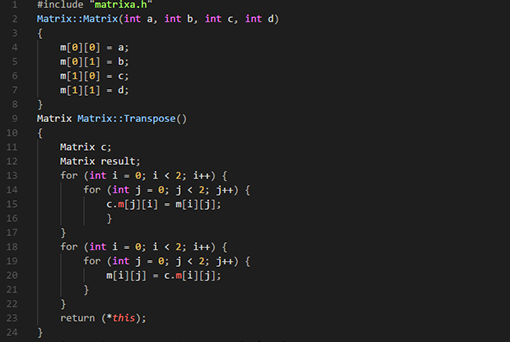
\includegraphics[width=1.0\columnwidth]{atrans}} 
\caption{matrixa.cpp의 Transpose 구현}\vspace*{-6pt} 
\label{figure:matrixa} 
\end{figure} 

\begin{figure}[t]\vspace*{4pt} 
\centerline{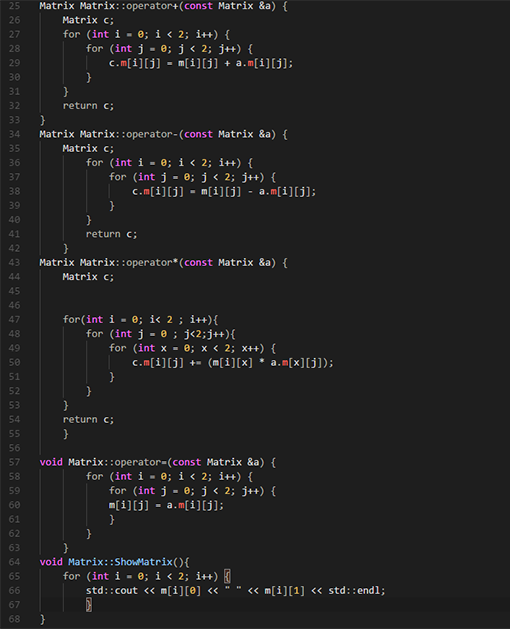
\includegraphics[width=1.0\columnwidth]{aother}} 
\caption{matrixa.cpp의 연산자 오버로딩}\vspace*{-6pt} 
\label{figure:matrixa_overload} 
\end{figure} 

\newpage
\begin{figure}[t]\vspace*{4pt} 
\centerline{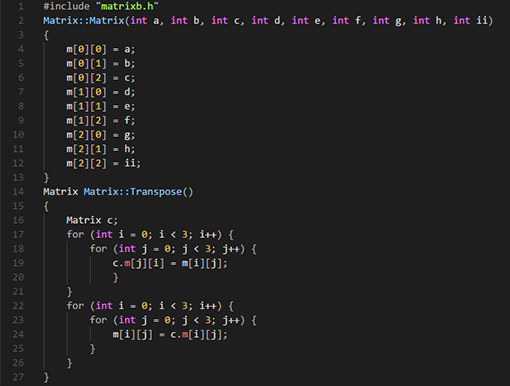
\includegraphics[width=1.0\columnwidth]{btrans}} 
\caption{matrixb.cpp의 Transpose 구현}\vspace*{-6pt} 
\label{figure:matrixb} 
\end{figure} 

\begin{figure}[t]\vspace*{4pt} 
\centerline{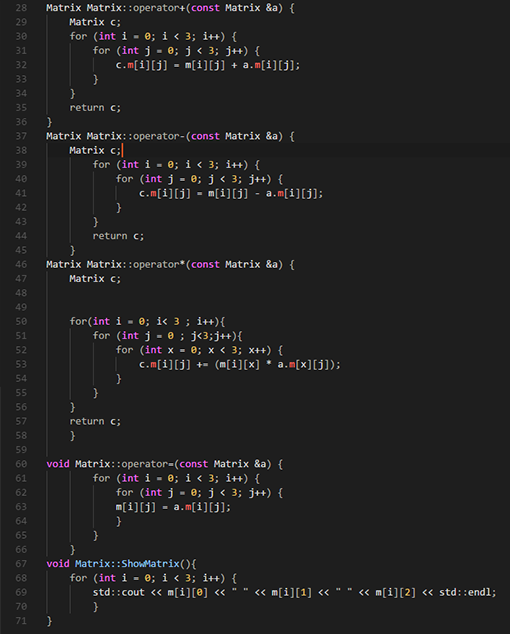
\includegraphics[width=1.0\columnwidth]{bother}} 
\caption{matrixb.cpp의 연산자 오버로딩}\vspace*{-6pt} 
\label{figure:matrixb_overload} 
\end{figure} 



\end{document} 